\section{Introduction}

Human children possess the remarkable capability to learn a new concept from just one or a
handful of examples. A child can easily learn simple visual concepts, like the word ``ball,"
after only seeing one or two balls.
In contrast, the best artificial learning systems require many thousands of examples
in order to effectively learn simple concepts.
%Although human behavioral studies offer ample evidence
%of inductive biases, little is known about how these biases are implemented
%in biological information processing systems.
\begin{figure}[h!]
    \begin{center}
        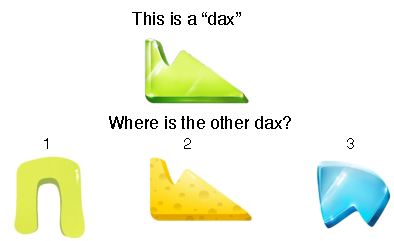
\includegraphics[width=0.3\textwidth]{figures/shape_bias_demo.pdf}
    \end{center}
    \caption{The shape bias. Children learn that objects with the same name tend to have the
    same shape, and thus option 2 above is likely the right answer. This
    inductive bias helps with future word learning.}
    \label{fig:shape_bias_demo}
\end{figure}

\blfootnote{The source code repository for this paper is located at
\url{http://github.com/rfeinman/learning-to-learn}}